%----------------------------------------------------------------------------------------
%	PACKAGES AND OTHER DOCUMENT CONFIGURATIONS
%----------------------------------------------------------------------------------------

\documentclass[
	a4paper, % Page size
	fontsize=10pt, % Base font size
	twoside=true, % Use different layouts for even and odd pages (in particular, if twoside=true, the margin column will be always on the outside)
	%open=any, % If twoside=true, uncomment this to force new chapters to start on any page, not only on right (odd) pages
	%chapterentrydots=true, % Uncomment to output dots from the chapter name to the page number in the table of contents
	numbers=noenddot, % Comment to output dots after chapter numbers; the most common values for this option are: enddot, noenddot and auto (see the KOMAScript documentation for an in-depth explanation)
]{kaobook}

\documentclass[
	a4paper, % Page size
	fontsize=10pt, % Base font size
	twoside=true, % Use different layouts for even and odd pages (in particular, if twoside=true, the margin column will be always on the outside)
	%open=any, % If twoside=true, uncomment this to force new chapters to start on any page, not only on right (odd) pages
	%chapterentrydots=true, % Uncomment to output dots from the chapter name to the page number in the table of contents
	numbers=noenddot, % Comment to output dots after chapter numbers; the most common values for this option are: enddot, noenddot and auto (see the KOMAScript documentation for an in-depth explanation)
]{kaobook}

\usepackage{mathtools}
\usepackage{cancel}
% Choose the language
\ifxetexorluatex
	\usepackage{polyglossia}
	\setmainlanguage{english}
\else
	\usepackage[english]{babel} % Load characters and hyphenation
\fi
\usepackage[english=british]{csquotes}	% English quotes

% Load packages for testing
\usepackage{blindtext}
%\usepackage{showframe} % Uncomment to show boxes around the text area, margin, header and footer
%\usepackage{showlabels} % Uncomment to output the content of \label commands to the document where they are used

% Load the bibliography package
\usepackage{kaobiblio}
\addbibresource{main.bib} % Bibliography file

% Load mathematical packages for theorems and related environments
\usepackage[framed=true]{kaotheorems}

% Load the package for hyperreferences
\usepackage{kaorefs}

\graphicspath{{examples/documentation/images/}{images/}} % Paths in which to look for images

\makeindex[columns=3, title=Alphabetical Index, intoc] % Make LaTeX produce the files required to compile the index

\makeglossaries % Make LaTeX produce the files required to compile the glossary
\newglossaryentry{computer}{
	name=computer,
	description={is a programmable machine that receives input, stores and manipulates data, and provides output in a useful format}
}

% Glossary entries (used in text with e.g. \acrfull{fpsLabel} or \acrshort{fpsLabel})
\newacronym[longplural={Frames per Second}]{fpsLabel}{FPS}{Frame per Second}
\newacronym[longplural={Tables of Contents}]{tocLabel}{TOC}{Table of Contents}

 % Include the glossary definitions

\makenomenclature % Make LaTeX produce the files required to compile the nomenclature

% Reset sidenote counter at chapters
%\counterwithin*{sidenote}{chapter}

% --------------------------------------------
% 		SOME MATH COMMANDS DEFINITIONS
% --------------------------------------------


\renewcommand{\d}{\text d} % differential
\newcommand{\dd}[2]{\dfrac{\d #1}{\d #2}} % total derivative 
\newcommand{\ddp}[2]{\dfrac{\partial #1}{\partial #2}} % partial derivative
\renewcommand{\vec}[1]{ \mathbf #1} % vectors with bold font
\newcommand{\abs}[1]{\lvert #1 \rvert} % absolute value
\newcommand{\del}{\partial} % del operator is not nabla
\newcommand{\paren}[1]{\left(#1\right)} % big parentheses
\newcommand{\commu}[2]{#1 #2 - #2 #1} % expansion of commutator
\newcommand{\ket}[1]{\lvert #1 \rangle} % ket
\newcommand{\bra}[1]{\langle #1 \rvert} % bra
\newcommand{\normbraket}[1]{\langle #1 \rvert #1 \rangle} % the norm of something in bra-ket notation
\newcommand{\then}{\Longrightarrow} % then arrow
%\newcommand{\def}{\coloneqq} % definition denoted as :=
\renewcommand{\mapsto}{\longmapsto} % long arrow for maps-to symbol
\newcommand{\reals}{\mathbb R} % set of real numbers
\newcommand{\complexes}{\mathbb C} % set of complex numbers

%----------------------------------------------------------------------------------------

\begin{document}

% --------------------------
%       PATH TO IMAGES
% --------------------------

\graphicspath{ 
    {chapters/Matemáticas/Sistema_de_coordenadas/images/}
    {images/}
}%

%----------------------------------------------------------------------------------------
%	BOOK INFORMATION
%----------------------------------------------------------------------------------------

\titlehead{PLNotes}
\subject{Use this document as a template}

\title[Physics Landscape - Notas]{Physics Landscape - Notas}
\subtitle{Notas de Física del grupo}

\author[et al.]{et al.}

\date{\today}

\publishers{Editorial PL}

%----------------------------------------------------------------------------------------

\frontmatter % Denotes the start of the pre-document content, uses roman numerals

%----------------------------------------------------------------------------------------
%	OPENING PAGE
%----------------------------------------------------------------------------------------

%\makeatletter
%\extratitle{
%	% In the title page, the title is vspaced by 9.5\baselineskip
%	\vspace*{9\baselineskip}
%	\vspace*{\parskip}
%	\begin{center}
%		% In the title page, \huge is set after the komafont for title
%		\usekomafont{title}\huge\@title
%	\end{center}
%}
%\makeatother

%----------------------------------------------------------------------------------------
%	COPYRIGHT PAGE
%----------------------------------------------------------------------------------------

\makeatletter
\uppertitleback{\@titlehead} % Header

\lowertitleback{
	\textbf{Disclaimer}\\
	You can edit this page to suit your needs. For instance, here we have a no copyright statement, a colophon and some other information. This page is based on the corresponding page of Ken Arroyo Ohori's thesis, with minimal changes.
	
	\medskip
	
	\textbf{No copyright}\\
	\cczero\ This book is released into the public domain using the CC0 code. To the extent possible under law, I waive all copyright and related or neighbouring rights to this work.
	
	To view a copy of the CC0 code, visit: \\\url{http://creativecommons.org/publicdomain/zero/1.0/}
	
	\medskip
	
	\textbf{Colophon} \\
	This document was typeset with the help of \href{https://sourceforge.net/projects/koma-script/}{\KOMAScript} and \href{https://www.latex-project.org/}{\LaTeX} using the \href{https://github.com/fmarotta/kaobook/}{kaobook} class.
	
	The source code of this book is available at:\\\url{https://github.com/fmarotta/kaobook}
	
	(You are welcome to contribute!)
	
	\medskip
	
	\textbf{Publisher} \\
	First printed in May 2019 by \@publishers
}
\makeatother

%----------------------------------------------------------------------------------------
%	DEDICATION
%----------------------------------------------------------------------------------------

\dedication{
	What we observe is not nature itself, but nature exposed to our method of questioning.\\\flushright Werner Heisenberg
}

%----------------------------------------------------------------------------------------
%	OUTPUT TITLE PAGE AND PREVIOUS
%----------------------------------------------------------------------------------------

% Note that \maketitle outputs the pages before here

\maketitle

%----------------------------------------------------------------------------------------
%	PREFACE
%----------------------------------------------------------------------------------------

\chapter*{Preface}
\addcontentsline{toc}{chapter}{Preface} % Add the preface to the table of contents as a chapter

La intención de las presentes notas es convertirse en un texto completo de física, incluyendo varios tópicos de nivel pregrado y grado, en idioma español. 
\index{preface}

%----------------------------------------------------------------------------------------
%	TABLE OF CONTENTS & LIST OF FIGURES/TABLES
%----------------------------------------------------------------------------------------

\begingroup % Local scope for the following commands

% Define the style for the TOC, LOF, and LOT
%\setstretch{1} % Uncomment to modify line spacing in the ToC
%\hypersetup{linkcolor=blue} % Uncomment to set the colour of links in the ToC
\setlength{\textheight}{230\hscale} % Manually adjust the height of the ToC pages

% Turn on compatibility mode for the etoc package
\etocstandarddisplaystyle % "toc display" as if etoc was not loaded
\etocstandardlines % "toc lines" as if etoc was not loaded

\tableofcontents % Output the table of contents

\listoffigures % Output the list of figures

% Comment both of the following lines to have the LOF and the LOT on different pages
\let\cleardoublepage\bigskip
\let\clearpage\bigskip

\listoftables % Output the list of tables

\endgroup

%----------------------------------------------------------------------------------------
%	MAIN BODY
%----------------------------------------------------------------------------------------

\mainmatter % Denotes the start of the main document content, resets page numbering and uses arabic numbers
\setchapterstyle{kao} % Choose the default chapter heading style

\pagelayout{wide} % No margins
\addpart{Mecánica Estadística} %% Part
\pagelayout{margin} % Restore margins

\pagelayout{wide} % No margins
\addpart{Mecánica Cuántica} %% Part
\pagelayout{margin} % Restore margins

\setchapterpreamble[u]{\margintoc}
\chapter{Momento Angular}
\labch{momento_angular}

Se define clásicamente como el producto cruz $\vec L = \vec r \times \vec p$. La k-ésima componente de este vector está dada por $L_k = \{\vec L\}_k = \epsilon _{ijk} r_i p_j$.

En mecánica clásica se sustituyen las cantidades por operadores $\vec L \rightarrow \hat{\vec L}$ 

% ---------------------
%       SECTIONS 
% ---------------------

\section{Relaciones de conmutación}
\subsection{Relación canónica: Posición y momento}
Se mostrará que $[x_i,p_j] = i\hbar\delta_{ij}$.

Recordando que $p_j = -i \hbar \ddp{}{x_j} = -i\hbar \del_j$, se tiene

\begin{align}
	[x_i, p_j] &= -i\hbar [x_i, \del_j] \\
			&= -i\hbar \paren{x_i \del_j - (\del_jx_i)}
\end{align}

Para ver más claramente en qué resulta de esta diferencia, se aplica la expresión a una función arbitraria $\psi$  
%(See [[Functions space#Calculation Example: $[X, D_{x}]$]])

\begin{align}
	\paren{x_i \del_j - (\del_jx_i)}\psi &= x_i \del_j\psi - \del_j(x_i \psi) \\
		&= x_i \del_j\psi - (\del_j x_i) \psi - x_i \del_j \psi \\
		&= -\delta_{ij}\psi
\end{align}

Finalmente, 
\begin{align}
	[x_i, p_j]\psi &= -i\hbar\paren{-\delta_{ij}\psi} \\
	\Rightarrow \Aboxed{[x_i, p_j] &= i\hbar\delta_{ij}}
\end{align}

\subsection{Momento Angular}
\subsubsection{$[L_i,L_j] = L_k$}


\begin{align}
	[L_i,L_j] &= [ \epsilon_{ist}x_s p_t , \epsilon_{jmn}x_m p_n ] \\
		&= \epsilon_{ist}\epsilon_{jmn}[ x_s p_t , x_m p_n ] \\
\end{align}

Se expande el último conmutador de la siguiente forma, 

\begin{align*}
	[ x_s p_t, x_m p_n ] &= x_s [  p_t, x_m p_n ] + [ x_s, x_m p_n ] p_t\\
		&= x_s x_m \cancel{[  p_t, p_n ]} + x_s [  p_t, x_m ]p_n  + x_m [ x_s, p_n ] p_t + \cancel{[ x_s, x_m ]}p_n p_t \\
		&= -x_s [x_m, p_t]p_n + x_m[ x_s, p_n]p_t \\
		&= -x_s(\delta_{mt})p_n + x_m(\delta_{sn})pt \\
		&= i\hbar \paren{x_m p_t \delta_{sn} - x_s p_n \delta_{mt}}
\end{align*}

Volviendo a la expresión completa,   

\begin{align}
	[L_i,L_j] &=i\hbar\epsilon_{ist}\epsilon_{jmn} \paren{x_m p_t \delta_{sn} - x_s p_n \delta_{mt}} \\
		&=i\hbar \paren{\epsilon_{ist}\epsilon_{jmn}x_m p_t \delta_{sn} - \epsilon_{ist}\epsilon_{jmn}x_s p_n \delta_{mt}}
\end{align}

Ahora, usando 

\begin{align*}
	[L_i,L_j] &= i\hbar\paren{\det\paren{\begin{bmatrix}
	\delta_{tj}&\delta_{tm}\\\delta_{ij}&\delta_{im}
	\end{bmatrix}}x_m p_t - \det\paren{\begin{bmatrix}
	\delta_{in}&\delta_{ij}\\\delta_{sn}&\delta_{sj}
	\end{bmatrix}}x_s p_n} \\
	&= i\hbar\paren{\paren{\delta_{tj}\delta_{im} - \delta_{ij}\delta_{tm}}x_m p_t - \paren{\delta_{in}\delta_{sj} - \delta_{sn}\delta_{ij}}x_sp_n} \\
	&= i\hbar \paren{x_i p_j - \cancel{x_tp_t\delta_{ij}} - x_jp_i + \cancel{x_s p_s\delta_{ij}}} \\
	&=  i\hbar \paren{x_i p_j -  x_jp_i } \\
	&= i\hbar \epsilon_{ijk} \,x_i p_j \\
	&= i\hbar\epsilon_{ijk}L_k
\end{align*}

\subsubsection{$[\vec L^2,L_k] = 0$}

\begin{align*}
	[\vec L^2,L_k] &= [L_i L_i,L_k] \\
		&= L_i[L_i,L_k] + [L_i,L_k]L_i \\
		&= i\hbar \paren{\epsilon_{ijk} L_i L_k + \epsilon_{ijk}L_k L_i} \\
		&= i\hbar\epsilon_{ijk}\{L_i,L_k\}
\end{align*}

El anticonmutador $\{\, ,\,\}$ es simétrico, cuando este se contrae con el tensor de Levi-Civital, el cual es antisimétrico, el resultado es nulo. 
%TODO show contraction of symmetric and antisymmetric tensors



# theorems about commuting operators


> [!Theorem 1]
> If two operators $A$ and $B$ commute, and if $\ket{\psi}$ is an eigenvector of $A$. Then $B \ket{\psi}$ is also an eigenvector of $A$ with the same eigenvalue.

> [!Proof 1] 
> Since $\ket{\psi}$ is eigenvector of $A$ it satisfies $A\ket{\psi} = a\ket{\psi}$. Apliying $B$ over the state on both sides one gets $BA\ket{\psi} = aB\ket{\psi}$. By hypothesis $AB = BA$, then $A(B\ket{\psi}) = a(B\ket{\psi})$. This last one means that the state $\ket{\phi} = B\ket{\psi}$ is eigenvector of $A$ with eigenvalue $a$.
> In the case $a$ is non-degenerate...
> #TODO continue with the proof

> [!Theorem 2]
> If two operators $A$ and $B$ commute, and if $\ket{ \psi_{1}}$ and $\ket{ \psi_{2}}$ are two eigenvectors of $A$ with different eigenvalues, the matrix element $\braketB{B}{\psi_{1}}{\psi_{2}}$ is zero.

> [!Proof 2]
> Contents


> [!Theorem 3]
> If two observables $A$ and $B$ commute, one can construct an orthonormal basis of the state space with eigenvectors common to $A$ and $B$.

# References

[QM, Cohen - Ch 2](file:///home/gabo/Zotero/storage/7DZ9SFA4/Cohen-Tannoudji%20et%20al.%20-%202020%20-%20Quantum%20mechanics.%20Volume%201%20Basic%20concepts,%20tools.pdf)


 


\section{Eigenvalue equations}








\pagelayout{wide} % No margins
\addpart{Matemáticas}
\pagelayout{margin} % Restore margins

%\setchapterstyle{kao}
\setchapterpreamble[u]{\margintoc}
\chapter{Mathematics and Boxes}
\labch{mathematics}

\section{Theorems}

Despite most people complain at the sight of a book full of equations, 
mathematics is an important part of many books. Here, we shall 
illustrate some of the possibilities. We believe that theorems, 
definitions, remarks and examples should be emphasised with a shaded 
background; however, the colour should not be to heavy on the eyes, so 
we have chosen a sort of light yellow.\sidenote{The boxes are all of the 
same colour here, because we did not want our document to look like 
\href{https://en.wikipedia.org/wiki/Harlequin}{Harlequin}.}

\begin{definition}
\labdef{openset}
Let $(X, d)$ be a metric space. A subset $U \subset X$ is an open set 
if, for any $x \in U$ there exists $r > 0$ such that $B(x, r) \subset 
U$. We call the topology associated to d the set $\tau\textsubscript{d}$ 
of all the open subsets of $(X, d).$
\end{definition}

\refdef{openset} is very important. I am not joking, but I have inserted 
this phrase only to show how to reference definitions. The following 
statement is repeated over and over in different environments.

\begin{theorem}
A finite intersection of open sets of (X, d) is an open set of (X, d), 
i.e $\tau\textsubscript{d}$ is closed under finite intersections. Any 
union of open sets of (X, d) is an open set of (X, d).
\end{theorem}

\begin{proposition}
A finite intersection of open sets of (X, d) is an open set of (X, d), 
i.e $\tau\textsubscript{d}$ is closed under finite intersections. Any 
union of open sets of (X, d) is an open set of (X, d).
\end{proposition}

\marginnote{You can even insert footnotes inside the theorem 
environments; they will be displayed at the bottom of the box.}

\begin{lemma}
A finite intersection\footnote{I'm a footnote} of open sets of (X, d) is 
an open set of (X, d), i.e $\tau\textsubscript{d}$ is closed under 
finite intersections. Any union of open sets of (X, d) is an open set of 
(X, d).
\end{lemma}

You can safely ignore the content of the theorems\ldots I assume that if 
you are interested in having theorems in your book, you already know 
something about the classical way to add them. These example should just 
showcase all the things you can do within this class.

\begin{corollary}[Finite Intersection, Countable Union]
A finite intersection of open sets of (X, d) is an open set of (X, d), 
i.e $\tau\textsubscript{d}$ is closed under finite intersections. Any 
union of open sets of (X, d) is an open set of (X, d).
\end{corollary}

\begin{proof}
The proof is left to the reader as a trivial exercise. Hint: \blindtext
\end{proof}

\begin{definition}
Let $(X, d)$ be a metric space. A subset $U \subset X$ is an open set 
if, for any $x \in U$ there exists $r > 0$ such that $B(x, r) \subset 
U$. We call the topology associated to d the set $\tau\textsubscript{d}$ 
of all the open subsets of $(X, d).$
\end{definition}

\marginnote{
	Here is a random equation, just because we can:
	\begin{equation*}
  x = a_0 + \cfrac{1}{a_1
          + \cfrac{1}{a_2
          + \cfrac{1}{a_3 + \cfrac{1}{a_4} } } }
	\end{equation*}
}

\begin{example}
Let $(X, d)$ be a metric space. A subset $U \subset X$ is an open set 
if, for any $x \in U$ there exists $r > 0$ such that $B(x, r) \subset 
U$. We call the topology associated to d the set $\tau\textsubscript{d}$ 
of all the open subsets of $(X, d).$
\end{example}

\begin{remark}
Let $(X, d)$ be a metric space. A subset $U \subset X$ is an open set 
if, for any $x \in U$ there exists $r > 0$ such that $B(x, r) \subset 
U$. We call the topology associated to d the set $\tau\textsubscript{d}$ 
of all the open subsets of $(X, d).$
\end{remark}

As you may have noticed, definitions, example and remarks have 
independent counters; theorems, propositions, lemmas and corollaries 
share the same counter.

\begin{remark}
Here is how an integral looks like inline: $\int_{a}^{b} x^2 dx$, and 
here is the same integral displayed in its own paragraph:
\[\int_{a}^{b} x^2 dx\]
\end{remark}

There is also an environment for exercises.

\begin{exercise}
Prove (or disprove) the Riemann hypothesis.
\end{exercise}

We provide one package for the theorem styles: 
\href{kaotheorems.sty}{kaotheorems.sty}, to which you can pass the 
\Option{framed} option you do want coloured boxes around theorems, like 
in this document.\sidenote{The styles without \Option{framed} are not 
showed, but actually the only difference is that they don't have the 
yellow boxes.} You may want to edit this files according to your taste 
and the general style of the book. However, there is an option to 
customise the background colour of the boxes if you use the 
\Option{framed} option: when you load this package, you can pass it the 
\Option{background=mycolour} option (replace \enquote{mycolour} with the 
actual colour, for instance, \enquote{red!35!white}). This will change 
the colour of all the boxes, but it is also possible to override the 
default colour only for some elements. For instance, the 
\Option{propositionbackground=mycolour} option will change the colour 
for propositions only. There are similar options for theorem, 
definition, lemma, corollary, remark, and example.

\section[Boxes \& Environments]{Boxes \& Custom Environments
\sidenote[][*1.8]{Notice that in the table of contents and in the 
	header, the name of this section is \enquote{Boxes \& Environments}; 
	we achieved this with the optional argument of the \texttt{section} 
	command.}}

Say you want to insert a special section, an optional content or just 
something you want to emphasise. We think that nothing works better than 
a box in these cases. We used \Package{mdframed} to construct the ones 
shown below. You can create and modify such environments by editing the 
provided file \href{style/environments.sty}{environments.sty}.

\begin{kaobox}[frametitle=Title of the box]
\blindtext
\end{kaobox}

If you set up a counter, you can even create your own numbered 
environment.

\begin{kaocounter}
	\blindtext
\end{kaocounter}

\section{Experiments}

It is possible to wrap marginnotes inside boxes, too. Audacious readers 
are encouraged to try their own experiments and let me know the 
outcomes.

\marginnote[-2.2cm]{
	\begin{kaobox}[frametitle=title of margin note]
		Margin note inside a kaobox.\\
		(Actually, kaobox inside a marginnote!)
	\end{kaobox}
}

I believe that many other special things are possible with the 
\Class{kaobook} class. During its development, I struggled to keep it as 
flexible as possible, so that new features could be added without too 
great an effort. Therefore, I hope that you can find the optimal way to 
express yourselves in writing a book, report or thesis with this class, 
and I am eager to see the outcomes of any experiment that you may try.

%\begin{margintable}
	%\captionsetup{type=table,position=above}
	%\begin{kaobox}
		%\caption{caption}
		%\begin{tabular}{ |c|c|c|c| }
			%\hline
			%col1 & col2 & col3 \\
			%\hline
			%\multirow{3}{4em}{Multiple row} & cell2 & cell3 \\ & cell5 
			%%& cell6 \\ 
			%& cell8 & cell9 \\
			%\hline
		%\end{tabular}
	%\end{kaobox}
%\end{margintable}


\setchapterpreamble[u]{\margintoc}
\chapter{Álgebra Tensorial Afín}
\labch{algebra_tensorial_afin}

\section{Introducción}

Puesto que en el contexto del viejo lenguaje, los tensores están relacionados con la conducta de diferentes entidades bajo el paso de un sistema de coordenadas a otro, comenzaremos con un análisis detallado del tipo más simple de transformación de coordenadas a saber, la transformación ortogonal en un espacio de coordenadas tridimensionales. Las propiedades de transformación de las componentes de vectores sugieren la introducción de una clase especial de tensores, los así llamados  **tensores afin**, cuya definición es formulada en términos de la conducta de sus componentes bajo transformaciones ortogonales en $E_3$. Ésta da lugar a una simple teoría algebraica de tensores que puede ser considerada como una extensión inmediata del álgebra vectorial elemental. Además las definiciones son de naturaleza tal que permiten una exitosa trancisión desde 3 a $n$ dimensiones.

Sin embargo, por definición, las transformaciones ortogonales son lineales, y consecuentemente la teoría de tensores afin es también una teoría restringida para muchos propósitos. Por ejemplo, cuando son introducidas coordenadas curvilíneas, uno está conformado por coordenadas que son nolineales. Por abstracción de algunas características del álgebra tensorial afin, uno puede formular de una manera natural una definición más general del concepto de tensor que sea independiente de la linealidad inherente en las transformaciones ortogonales. Una aplicación inmediata de estas ideas es el estudio de campos vectoriales paralelos en $E_n$ referidos a coordenadas curvilineas

\section{Transformaciones ortogonales en $E_3$}

Consideremos una transformación desde un sistema de coordenada rectangular a otro, asumiendo que estos sistemas tienen un origen común en el punto $O$ de espacio euclídeono tridimensional $E_3$. Los vectores unitarios en las direcciones positivas de los ejes $OX^1$,$OX^2$,$OX^3$ son denotados por $\vec{e_1}$,$\vec{e}_2$,$\vec{e_3}$

\begin{equation}
  \vec{e_i}\cdot\vec{e_j}=\delta_{ij} \hspace{3cm}(i,j=1,2,3)
  \label{eq:eq_1}
\end{equation}

Es decir que los vectores $\vec{e_i}$ constituyen una base ortonormal de $E_3$, lo cual significa que cualquier vector de $E_3$ puede ser expresado como una combinación lineal de los vectores bases. En particular, para los vectores bases de otra base ortonormal centrada en $O$, denotada por $\vec{f_i}$   ($i=1,2,3$), podemos escribir:

\begin{eqnarray*}
  \begin{array}{c}
    \vec{f_1}=a_11\vec{e_1}+a_12\vec{e_2}+a_13\vec{e_3} \\
    \vec{f_2}=a_21\vec{e_1}+a_22\vec{e_2}+a_23\vec{e_3} \\
    \vec{f_3}=a_31\vec{e_1}+a_32\vec{e_2}+a_33\vec{e_3}
  \end{array}
  &\Rightarrow&
  \begin{array}{lcr}
    \begin{pmatrix}{c}
      \vec{f_1}\\
      \vec{f_2}\\
      \vec{f_3}
    \end{pmatrix}

     & = &
    \begin{pmatrix}{c c c}
      a_11 & a_12 & a_13 \\
      a_21 & a_22 & a_23 \\
      a_31 & a_32 & a_33
    \end{pmatrix}
    \begin{pmatrix}{c}
      \vec{e_1} \\
      \vec{e_2} \\
      \vec{e_3}
    \end{pmatrix}
  \end{array}
\end{eqnarray*}

Donde los $a_{ik}$ son parámetros reales que dependen de la dirección de los vectores $\vec{f_i}$ con respecto a las bases $\{\vec{e_j}\}$.

De modo más compacto podemos escribir

$$\vec{f_j}=\sum^{3}_{i=1}a_{ji}\vec{e_i}$$

Claramente esta transformación es caracterizada completamente por la matriz de $3\times 3 (a_{ik})$, cuyos elementos poseen una simple interpretación geométrica: Cuando los productos escalares de $\vec{f_j}$ con $\vec{e_k}$ son construidos y la relación \eqref{eq:eq_1} es tomada en cuenta tenemos:

$$ 
\vec{f_j}\cdot\vec{e_k}=\sum^{3}_{i=1}a_{ji}\vec{e_i}\cdot=\sum^{3}_{i=1}a_{ji}\delta_{ik}=a_{jk}
$$

\begin{equation}
    \vec{f_j}\cdot\vec{e_k}=a_{jk}
    \label{eq:eq_3}
  \end{equation}
y puesto que $\vec{f_j}$ y $\vec{e_j}$ son vectores unitarios, tenemos:
$$a_{jk}=\vec{f_j}\cdot\vec{e_k}=\mid\vec{f_j}\mid\mid\vec{e_k}\mid\cos(\vec{f_j},\vec{e_k})\hspace{2 cm}
$$

\begin{equation}
  a_{jk}=\cos(\vec{f_j},\vec{e_k})\hspace{2cm}(j,k=1,2,3)
  \label{eq:eq_4}
\end{equation}

De modo que los coeficientes $a_{jk}$ en \eqref{eq:eq_3} son simplemente los cosenos de los ángulos entre los diferentes vectores bases de dos sistemas ortonormales, lo cual implica que los $a_{jk}$ no pueden asumir valores arbitrarios ser independientes uno de los otros. En realidad existe un conjunto de relación entre ellos el que puede ser obtenido como sigue:
Para la base ortonormal $\{\vec{f_j}\}$ se tiene
$$
  \vec{f_i}\cdot\vec{f_j}=\delta_{ij}\hspace{3 cm}
$$
de modo que, de acuerdo con (2)
\begin{eqnarray*}
    \delta_{jk}&=&\left[\sum^{3}_{i=1}a_{ji}\vec{e_i}\right]\left[\sum^{3}_{l=1}a_{hl}\vec{e_l}\right]=\sum^{3}_{i=1}\sum^{3}_{l=1}a_{ji}a_{kl}(\vec{e_i}\vec{e_l})\\
    \delta_{jk}&=&\sum^{3}_{i=1}\sum^{3}_{l=1}a_{ji}a_{kl}\delta_{il}=\sum^{3}_{i=1}a_{ji}a_{ki}
  \end{eqnarray*}
\begin{equation}
  \delta_{jk}=\sum^{3}_{i=1}a_{ji}a_{ki}  
  \label{eq:eq_5}
\end{equation}
La traspuesta $a_{jl}$ de los elementos $a_{lj}$ de la matriz $(a_{lj})$ es denotada por $a^T_{lj}$, por lo que (5) puede ser escrita como
\begin{equation}
    \sum^{3}_{i=3}a_{ji}a^{T}_{ik}=\delta_{jk}\hspace{2 cm}(i,k=1,2,3)
    \label{eq:eq_5}
\end{equation}

Estas relaciones representan una condición necesria que deben satisfacer los coeficientes $a_{ji}$ en (2) para que (2) represente una transformación desde una base ortonormal a otra. Invirtiendo los argumentos es directo mostrar que (6) es también una condición suficiente. Cualquier transformación lineal que satisfaga (6) es llamado una transformación ortogonal y correspondiente matriz $(a_{ji})$ es llamada matriz ortogonal

$$(6)\hspace{1 cm}\leftrightarrow\hspace{1 cm} AA^T=I$$
Es evidente, de la definición de determinante que:
$$det(a^T_{ji})=det(a_{ij})$$
y por tanto
\begin{eqnarray*}
    det(a_{ji})det(a^T_{ik})=\left[det(a_{ij})\right]^2=det\delta_{ij}=1
  \end{eqnarray*}
de modo que el determinante de cualquier matriz ortogonal satisface la condición
\begin{equation}
    det(a_{ij})=\pm 1
    \label{eq:eq_7}
\end{equation}

De modo que $det(a_{ij})\neq0$, y por lo tanto a la inversa de la matriz $(a_{ij})$ existe. De (\ref{6}) vemos que la inversa de una matriz ortogonal es idéntica a su traspuesta
$$(a_{ij})^T=(a_{ij})^{-1}$$

Esto puede ser iludtrado por geometricamente por el hecho que la matriz de la transformación inversa de (2) es en efecto, la traspuesta de la matriz $(a_{ji})$ que caracteriza (2) multiplicando (2) por  $a^T_{kj}$ y luego sumando sobre $j$ de 1 a 3 y considerando (6) tenemos:

\begin{eqnarray*}
    \vec{f_j}=\sum^{3}_{i=3}a_{ji}\vec{e_i}&\hspace{1 cm}\lfloor\, a^T_{kj}\hspace{0.5 cm} \lfloor \sum_{j}\\
    \sum^{3}_{j=1}a^T_{ij}\vec{f_j}=\sum^{3}_{j=1}\sum^{3}_{i=1}a^T_{kj}a_{ji}\vec{e_i}=\sum^{3}_{i=3}\delta_{ki}\vec{e_i}&
\end{eqnarray*}

\begin{equation}
    \vec{e_k}=\sum^{3}_{j=1}a^{T}_{kj}\vec{f_j}
    \label{eq:eq_7}
\end{equation}

Esta relación expresa los vectoresbases $\vec{e_k}$ en términos de los $\vec{f_j}$ y representa el inverso de la transformación ortogonal (2). Además en la misma manera en que (2) de lugar a (4) tenemos:

$$
  \vec{e_k}\cdot\vec{f_i}=\sum^{3}_{j=1}a^T_{kj}\vec{f_j}\cdot\vec{f_i}=\sum^{3}_{j=1}a^T_{kj}\delta_{ji}=a^T_{ki}
$$

\begin{equation*}
    \Rightarrow \hspace{3 cm}a^T_{ki}=\vec{e_i}\vec{f_i}=\mid\vec{e_k}\mid\mid\vec{f_i}\mid\cos(\vec{e_k},\vec{f_i})\hspace{3 cm}
\end{equation*}

\begin{equation}
  \Rightarrow \hspace{2 cm}a^T_{ki}=cos(\vec{e_k},\vec{f_i})
  \label{eq:eq_7}
\end{equation}

Sea $\{\vec{g}_l\}$ la base de vectores de una tercera base ortogonal cuyo origen está localizado en O. Claramente cada vector $\vec{g}_l$ puede ser representado en términos de la base original:
Por ejemplo
\begin{equation}
  \vec{g}_l=\sum^{3}_{j=1}c_{lj}\vec{f}_{j}
\end{equation}

Usando (2) tenemos,

\begin{equation}
  \vec{g}_l=\sum^{3}_{i=1}\sum^{3}_{j=1}c_{lj}a_{ji}\vec{e}_{i}
  \label{eq:eq_11}
\end{equation}

De modo que si escribimos
\begin{equation}
  \vec{g}_l=\sum^{3}_{i=1}b_{li}\vec{e}_{i}
  \label{eq:eq_12}  
\end{equation}
tenemos
\begin{equation}
  b_{li}=\sum^{3}_{j=1}c_{lj}a_{ji}
  \label{eq:eq_13}
\end{equation}
la cual prueba que la matriz $b_{li}$ es el producto de las matrices $(c_{li})$ y $(a_{ji})$.

La transformación caractericazada por la matriz $b_{li}$ es llamada el producto de las transformaciones (10) y (2). Por lo tanto, puesto que $b_{li}$ es ortogonal por construcción, se sigue que el producto de cualquier par de transformaciones ortogonales es denuevo ortogonal. También, puesto que el producto de matrices satisface obviamente una ley asociativa, podemos inferir que el conjunto de todas las transformaciones ortogonales en $E_3$ está dotado con una operación binaria asociativa, a saber, el producto, el cual es tal que el producto de cualquier par de elementos es denuevo un elemento del conjunto. Además, este conjunto contiene un elemento unidad, definido como la transformación identidad cuyos coeficientes son deltas de kronecker, mientras que la existencia del inverso de cada elemento es asegurado. Así tenemos que el conjunto de todas las transformaciones ortogonales en $E_3$  forman un grupo llamado el grupo ortogonal usualmente denotado por $O(3)$
%\chapter{Coordenadas Curvilíneas Ortogonales }

Clase 1

Los sistemas de coordenadas curvilíneas ortogonales hacen referencia a puntos en el espacio determinados por el corte de tres superficies, tales que, los vectores unitarios tangentes a cada curva de la intersección de dos de ellos son ortogonales entre sí.

Como ejemplo, revisemos que ocurre en las coordenadas cartesianas. Allí, cada punto espacial es determinado por la intersección de tres planos mutuamente ortogonales entre sí y que adicionalmente los tres vectores unitarios $\hat{i}, \hat{j}, \hat{k}$ permanecerán siendo los mismos mediante una operación de traslación de ellos al punto en consideración.

\begin{center}
  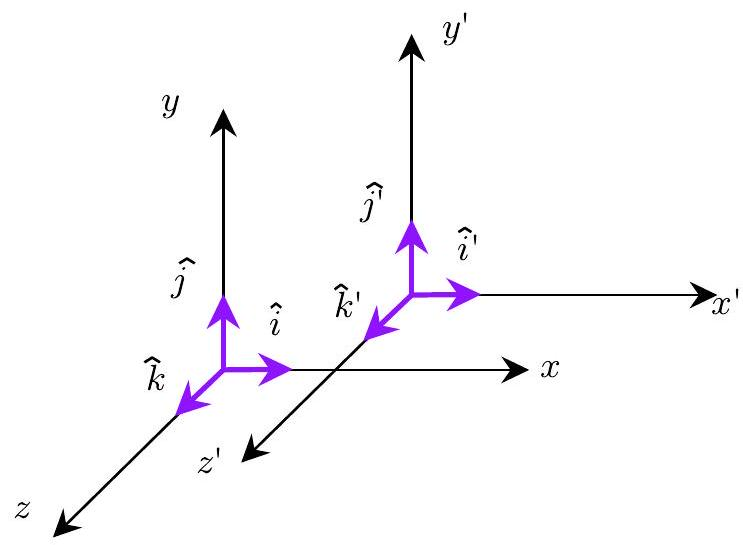
\includegraphics[max width=\textwidth]{sistemas_coordenados}
\end{center}

De tal forma que $\hat{i}=\hat{i}^{\prime}, \hat{j}=\hat{j}^{\prime}, \hat{k}=\hat{k}^{\prime}$

Miremos ahora que sucede en coordenadas cilíndricas. En este caso, las tres superficies que se intersectan son:

\begin{itemize}
  \item Un cilindro, un plano y un semiplano, De esta manera las tres nuevas variables serán: $\rho$ el radio del cilindro, $\theta$ el ángulo de apertura del semiplano y $z$ la posición del plano. Observemos esto en la siguiente figura:
\end{itemize}

\begin{center}
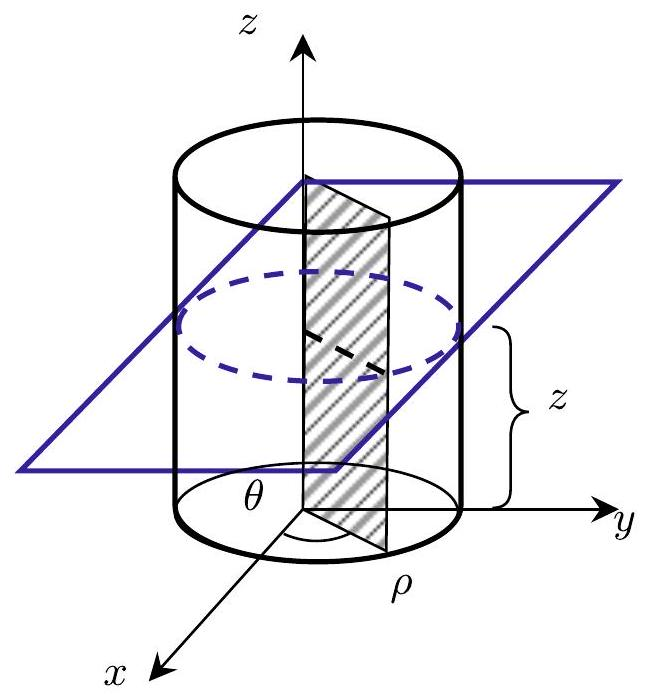
\includegraphics[max width=\textwidth]{coordenadas_colindricas.jpg}
\end{center}

Como se evidencia en la figura, la curva producto del corte entre el cilindro y el semiplano es una línea recta vertical, que determinará la coordenada $z$; la curva determinada por el corte del semiplano y el plano, determinará una semirecta que será $\rho$ y por último el corte entre el plano y el cilindro, será una circunferencia, que determinará $\theta$. De esta forma los tres vectores unitarios ortogonales entre sí y tangentes a estas curvas, serán:

$\hat{e}_{\rho}:$ vector tangente a la semirecta

$\hat{e}_{\theta}$ : vector tangente a la circunferencia

$\hat{e}_{z}$ : vector tangente a la recta vertical

Ellos forman entre sí un conjunto de mano derecha, por lo tanto

$$
\hat{e}_{\rho}=\hat{e}_{\theta} \times \hat{e}_{z}, \quad \hat{e}_{z}=\hat{e}_{\rho} \times \hat{e}_{\theta}, \quad \widehat{e}_{\theta}=\hat{e}_{z} \times \hat{e}_{\rho} .
$$

Adicionalmente, la propiedad de ortogonalidad la evidencio como:

$$
\widehat{e}_{\rho} \cdot \widehat{e}_{\theta}=\widehat{e}_{\rho} \cdot \widehat{e}_{z}=\widehat{e}_{\theta} \cdot \hat{e}_{z}=0
$$

Por último, como ejemplo, revisemos el caso de las coordenadas esféricas. En este caso las superficies que se intersectan son: una esfera, un semiplano y un tronco de cono.

Las respectivas curvas que se producen son:

\begin{itemize}
  \item De la intersección del tronco de cono y la esfera, una circunferencia.

  \item Del cono y el semiplano una semirecta.

  \item Del semiplano y la esfera, una semicircunferencia.

\end{itemize}

Lo que determina tres vectores unitarios ortogonales

$\hat{e}_{r}$ : vector tangente a la semirecta

$\hat{e}_{\theta}$ : vector tangente a la semicircunferencia

$\hat{e}_{\varphi}:$ vector tangente a la circunferencia

y las tres variables $r, \theta, \varphi$.

De nuevo este conjunto de vectores unitarios forman un conjunto de mano derecha, por lo tanto:

$$
\widehat{e}_{r}=\widehat{e}_{\theta} \times \hat{e}_{\varphi}, \hat{e}_{\varphi}=\widehat{e}_{r} \times \widehat{e}_{\theta}, \widehat{e}_{\theta}=\hat{e}_{\varphi} \times \hat{e}_{r}
$$

Debe notarse muy especialmente que en cualquier sistema de coordenadas curvilíneas ortogonales que no sea el cartesiano, la dirección de los vectores unitarios cambia punto a punto. Este hecho es importante, pues, mientras los vectores $\hat{i}, \hat{j}, \hat{k}$ no varían punto a punto, los otros si lo harán. Para los dos últimos casos mencionados debe tenerse en cuenta que las respectivas transformaciones de coordenadas entre estos sistemas y el cartesiano, son:

\begin{center}
\begin{tabular}{|l|l|}
\hline
Cilíndricas & Esféricas \\
\hline
\end{tabular}
\end{center}

$$
x=\rho \cos \theta, y=\rho \sin \theta, z
$$

$$
\begin{aligned}
& x=r \sin \theta \cos \varphi \\
& y=r \sin \theta \sin \varphi \\
& z=r \cos \theta
\end{aligned}
$$

Dentro del espacio Euclideo, se reconocen los siguientes sistemas de coordenadas curvilíneas ortogonales

\begin{center}
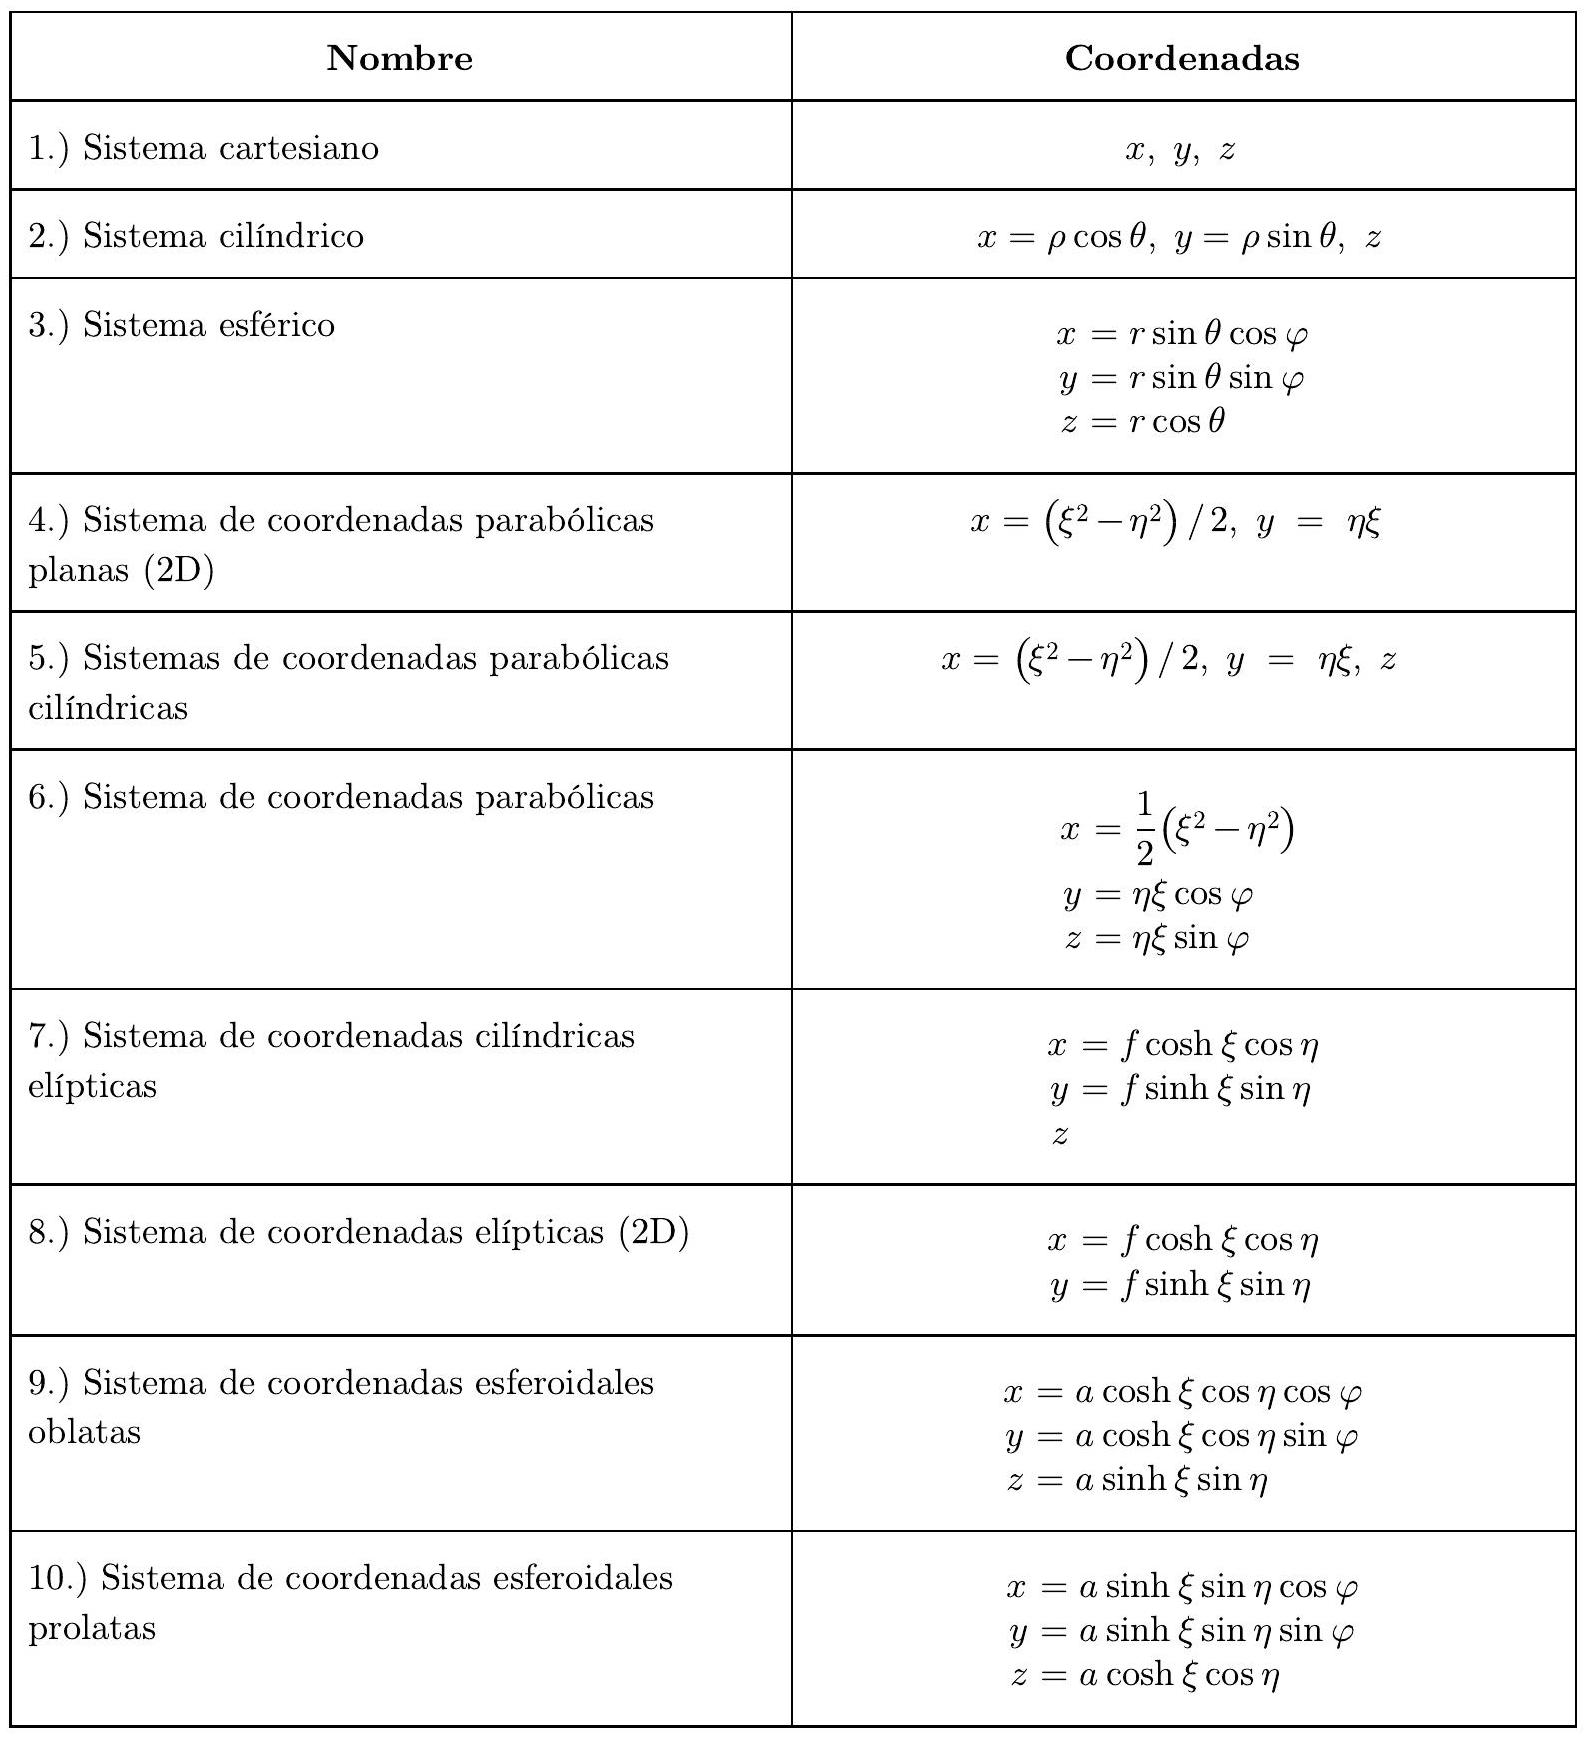
\includegraphics[max width=\textwidth]{tabla_sistemas_coordenados.jpg}
\end{center}

\begin{center}
\begin{tabular}{|l|l|}
\hline
11.) Sistema de coordenadas bipolares & $x=\frac{a \sinh \eta}{\cosh \eta-\cos \xi}$ \\
 & $y=\frac{a \sin \xi}{\cosh \eta-\cos \xi}$ \\
 & $z$ \\
\hline
12.) Sistema de coordenadas toroidales & $x=\frac{a \sinh \eta \cos \varphi}{\cosh \eta-\cos \xi}$ \\
 & $y=\frac{a \sinh \eta \sin \varphi}{\cosh \eta-\cos \xi}$ \\
 & $z=\frac{a \sin \xi}{\cosh \eta-\cos \xi}$ \\
\hline
13.) Sistema de coordenadas biesféricas & $y=\frac{a \sin \xi \cos \varphi}{\cosh \eta-\cos \xi}$ \\
 & $y=\frac{a \sin \xi \sin \varphi}{\cosh \eta-\cos \xi}$ \\
 & $z=\frac{a \sinh \eta}{\cosh \eta-\cos \xi}$ \\
\hline
\end{tabular}
\end{center}

Cada sistema coordenado tendrá un dominio para cada una de sus variables, de modo que queden cubiertos todos los puntos del plano o el espacio según sea la situación.

Consideremos ahora la siguiente situación general, si $x=x\left(u_{1}, u_{2}, u_{3}\right), y=y\left(u_{1}, u_{2}, u_{3}\right)$ y $z=z\left(u_{1}, u_{2}, u_{3}\right)$, del cálculo diferencial

$$
\begin{aligned}
& d x=\frac{\partial x\left(u_{1}, u_{2}, u_{3}\right)}{\partial u_{1}} d u_{1}+\frac{\partial x\left(u_{1}, u_{2}, u_{3}\right)}{\partial u_{2}} d u_{2}+\frac{\partial x\left(u_{1}, u_{2}, u_{3}\right)}{\partial u_{3}} d u_{3} \\
& d y=\frac{\partial y\left(u_{1}, u_{2}, u_{3}\right)}{\partial u_{1}} d u_{1}+\frac{\partial y\left(u_{1}, u_{2}, u_{3}\right)}{\partial u_{2}} d u_{2}+\frac{\partial y\left(u_{1}, u_{2}, u_{3}\right)}{\partial u_{3}} d u_{3} \\
& d z=\frac{\partial z\left(u_{1}, u_{2}, u_{3}\right)}{\partial u_{1}} d u_{1}+\frac{\partial z\left(u_{1}, u_{2}, u_{3}\right)}{\partial u_{2}} d u_{2}+\frac{\partial z\left(u_{1}, u_{2}, u_{3}\right)}{\partial u_{3}} d u_{3}
\end{aligned}
$$

De tal manera,

$$
\begin{aligned}
d \vec{r} & =\frac{\partial \vec{r}}{\partial u_{1}} d u_{1}+\frac{\partial \vec{r}}{\partial u_{2}} d u_{2}+\frac{\partial \vec{r}}{\partial u_{3}} d u_{3} \\
& =\sum_{i=1}^{3} \frac{\partial \vec{r}}{\partial u_{i}} d u_{i}
\end{aligned}
$$

Si se propone que: $\frac{\partial \vec{r}}{\partial u_{i}}=h_{i} \hat{e}_{i}$, entendiendo que la derivada de $\vec{r}$ se escribe en la base de vectores $\left\{\widehat{e}_{i}\right\}$ unitarios. De ahí desprendemos,

$$
h_{i}=\left|\frac{\partial \vec{r}}{\partial u_{i}}\right| \quad \hat{e}_{i}=\frac{1}{h_{i}} \frac{\partial \vec{r}}{\partial u_{i}}
$$

La constante de proporcionalidad $h_{i}$ recibe el nombre de factor de escala.

\section{Ejemplos:}
Encuentre los factores de escala y los vectores unitarios en coordenadas cilíndricas y esféricas.

Escribamos a $\vec{r}$ en coordenadas cartesianas

$$
\vec{r}=x \hat{i}+y \hat{j}+z \hat{k}
$$

Con la transformación: $x=\rho \cos \theta, y=\rho \sin \theta, z$

$$
\begin{aligned}
& \vec{r}=\rho \cos \theta \hat{i}+\rho \sin \theta \hat{j}+z \hat{k} \\
h_{\rho} & =\left|\frac{\partial}{\partial \rho}\{\rho \cos \theta \hat{i}+\rho \sin \theta \hat{j}+z \hat{k}\}\right| \\
= & |\cos \theta \hat{i}+\sin \theta \hat{j}| \\
= & \sqrt{\sin ^{2} \theta+\cos ^{2} \theta} \\
h_{\rho} & =1 \\
h_{\theta} & =\left|\frac{\partial}{\partial \theta}\{\rho \cos \theta \hat{i}+\rho \sin \theta \hat{j}+z \hat{k}\}\right| \\
= & \mid-\rho \sin \theta \hat{i}+\rho \cos \theta \hat{j}\rceil \\
& =\sqrt{\rho^{2}\left(\sin 2 \theta+\cos ^{2} \theta\right)} \\
h_{\theta} & =\rho \\
h_{z}= & \left|\frac{\partial}{\partial z}\{\rho \cos \theta \hat{i}+\rho \sin \theta \hat{j}+z \hat{k}\}\right| \\
& =|1 \hat{k}| \\
h_{z} & =1
\end{aligned}
$$

De esta manera los factores de escala en coordenadas cilíndricas, son:

$$
\left(h_{\rho}, h_{\theta}, h_{z}\right)=(1, \rho, 1)
$$

De acá los vectores unitarios, son: $\left(\widehat{e}_{i}=\frac{1}{h_{i}} \frac{\partial \vec{r}}{\partial u_{i}}\right)$

$$
\begin{aligned}
\widehat{e}_{\rho} & =\frac{1}{h_{\rho}} \frac{\partial \vec{r}}{\partial \rho} \\
& =\frac{\partial \vec{r}}{\partial \rho} \quad\left(\text { ya que } h_{\rho}=1\right) \\
& =\frac{\partial}{\partial \rho}\{\rho \cos \theta \hat{i}+\rho \sin \theta \hat{j}+z \hat{k}\} \\
\hat{e}_{\rho} & =\cos \theta \hat{i}+\sin \theta \hat{j}
\end{aligned}
$$

$$
\begin{aligned}
\hat{e}_{\theta} & =\frac{1}{h_{\theta}} \frac{\partial \vec{r}}{\partial \theta} \\
& =\frac{1}{\rho} \frac{\partial}{\partial \theta}\{\rho \cos \theta \hat{i}+\rho \sin \theta \hat{j}+z \hat{k}\} \\
\hat{e}_{\theta} & =-\sin \theta \hat{i}+\cos \theta \hat{j} \\
\widehat{e}_{z} & =\frac{1}{h_{z}} \frac{\partial \vec{r}}{\partial z} \\
& =\frac{\partial \vec{r}}{\partial z}\left(\text { ya que } h_{z}=1\right) \\
& =\frac{\partial}{\partial z}\{\rho \cos \theta \hat{i}+\rho \sin \theta \hat{j}+z \hat{k}\} \\
\hat{e}_{z} & =\hat{k}
\end{aligned}
$$

Por lo tanto

$$
\left\{\widehat{e}_{\rho}, \hat{e}_{\theta}, \hat{e}_{z}\right\}=\{\cos \theta \hat{i}+\sin \theta \hat{j},-\sin \theta \hat{i}+\cos \theta \hat{j}, \hat{k}\}
$$

De donde podemos constatar que:

$$
\begin{aligned}
\widehat{e}_{\rho} \cdot \hat{e}_{\theta} & =(\cos \theta \hat{i}+\sin \theta \hat{j}) \cdot(-\sin \theta \hat{i}+\cos \theta \hat{j}) \\
& =-\sin \theta \cos \theta+\sin \theta \cos \theta \\
& =0 \\
\hat{e}_{\rho} \cdot \widehat{e}_{z} & =(\cos \theta \hat{i}+\sin \theta \hat{j}) \cdot(\hat{k}) \\
& =0 \\
\widehat{e}_{\theta} \cdot \hat{e}_{z} & =(-\sin \theta \hat{i}+\cos \theta \hat{j}) \cdot(\hat{k}) \\
& =0
\end{aligned}
$$

$\mathrm{Y}$

$$
\begin{aligned}
& \hat{e}_{\rho} \cdot \hat{e}_{\rho}=(\cos \theta \hat{i}+\sin \theta \hat{j}) \cdot(\cos \theta \hat{i}+\sin \theta \hat{j}) \\
& =\cos ^{2} \theta+\sin ^{2} \theta \\
& =1 \\
& \widehat{e}_{\theta} \cdot \hat{e}_{\theta}=(-\sin \theta \hat{i}+\cos \theta \hat{j}) \cdot(-\sin \theta \hat{i}+\cos \theta \hat{j}) \\
& =\sin ^{2} \theta+\cos ^{2} \theta \\
& =1 \\
& \hat{e}_{z} \cdot \hat{e}_{z}=(\hat{k}) \cdot(\widehat{k}) \\
& =1
\end{aligned}
$$

Lo cual muestra que se tiene una base de vectores unitarios y ortogonales $\left(\hat{e}_{\rho}, \hat{e}_{\theta}, \hat{e}_{z}\right)$. También se puede verificar que es un sistema de mano derecha. Verifiquemos que $\widehat{e}_{\rho}=\hat{e}_{\theta} \times \hat{e}_{z}$

$$
\begin{aligned}
\hat{e}_{\theta} \times \widehat{e}_{z} & =\left|\begin{array}{ccc}
\hat{i} & \hat{j} & \hat{k} \\
-\sin \theta & \cos \theta & 0 \\
0 & 0 & 1
\end{array}\right| \\
& =(\cos \theta-0) \hat{i}-(-\sin \theta-0) \hat{j}+(0-0) \hat{k} \\
& =\cos \theta \hat{i}+\sin \theta \hat{j}
\end{aligned}
$$

Como $\hat{e}_{\rho}=\cos \theta \hat{i}+\sin \theta \hat{j}$, entonces

$$
\hat{e}_{\rho}=\hat{e}_{\theta} \times \hat{e}_{z}
$$

De manera análoga:

$$
\hat{e}_{\theta}=\widehat{e}_{z} \times \widehat{e}_{\rho}
$$

Calculemos:

$$
\begin{aligned}
\hat{e}_{z} \times \hat{e}_{\rho} & =\left|\begin{array}{ccc}
\hat{i} & \hat{j} & \hat{k} \\
0 & 0 & 1 \\
\cos \theta & \sin \theta & 0
\end{array}\right| \\
& =(0-\sin \theta) \hat{i}-(0-\cos \theta) \hat{j}+(0-0) \hat{k} \\
& =-\sin \theta \hat{i}+\cos \theta \hat{j}
\end{aligned}
$$

Como $\hat{e}_{\theta}=-\sin \theta \hat{i}+\cos \theta \hat{j}$, entonces se ha verificado que: $\hat{e}_{\theta}=\hat{e}_{z} \times \hat{e}_{\rho}$.

Finalmente verifiquemos que: $\widehat{e}_{z}=\widehat{e}_{\rho} \times \widehat{e}_{\theta}$

$$
\begin{aligned}
\widehat{e}_{\rho} \times \widehat{e}_{\theta} & =\left|\begin{array}{ccc}
\hat{i} & \hat{j} & \hat{k} \\
\cos \theta & \sin \theta & 0 \\
-\sin \theta & \cos \theta & 0
\end{array}\right| \\
& =(0-0) \hat{i}-(0-0) \hat{j}+\left(\cos ^{2} \theta+\sin ^{2} \theta\right) \hat{k} \\
& =\widehat{k}
\end{aligned}
$$

Por lo tanto $\hat{e}_{z}=\hat{e}_{\rho} \times \hat{e}_{\theta}$

\section{Tarea:}
\begin{itemize}
  \item Realizar todo lo anterior para las coordenadas esféricas, es decir, encontrar factores de escala, vectores unitarios, probar su ortogonalidad, unitariedad y regla de la mano derecha.

  \item Tomar las coordenadas esferoidales oblatas y hacer todo lo anterior.

\end{itemize}


\begin{center}
	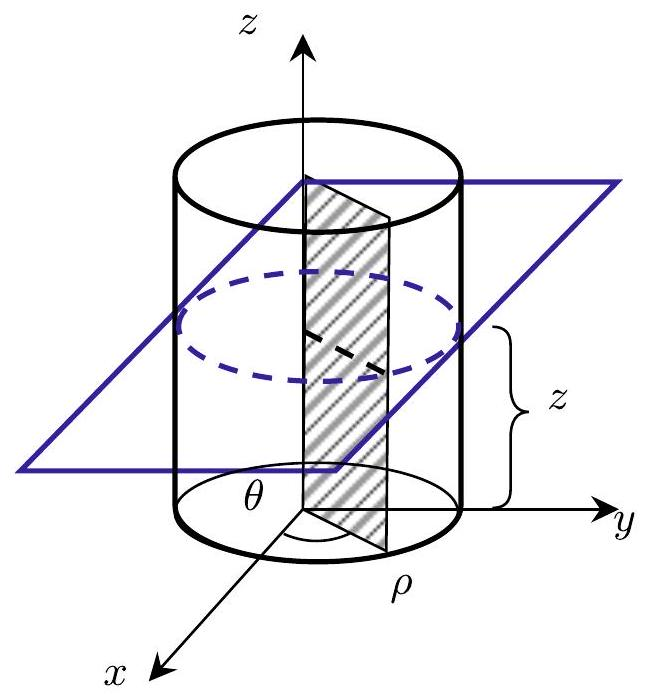
\includegraphics[]{cord_cilindricas}
\end{center}

\pagelayout{wide} % No margins
\addpart{Cosmología}
\pagelayout{margin} % Restore margins

%\input{chapters/Cosmología/Espacios simétricos.tex}
\appendix % From here onwards, chapters are numbered with letters, as is the appendix convention

\pagelayout{wide} % No margins
\addpart{Appendix}
\pagelayout{margin} % Restore margins



%----------------------------------------------------------------------------------------

\backmatter % Denotes the end of the main document content
\setchapterstyle{plain} % Output plain chapters from this point onwards

%----------------------------------------------------------------------------------------
%	BIBLIOGRAPHY
%----------------------------------------------------------------------------------------

% The bibliography needs to be compiled with biber using your LaTeX editor, or on the command line with 'biber main' from the template directory

\defbibnote{bibnote}{Here are the references in citation order.\par\bigskip} % Prepend this text to the bibliography
\printbibliography[heading=bibintoc, title=Bibliography, prenote=bibnote] % Add the bibliography heading to the ToC, set the title of the bibliography and output the bibliography note

%----------------------------------------------------------------------------------------
%	NOMENCLATURE
%----------------------------------------------------------------------------------------

% The nomenclature needs to be compiled on the command line with 'makeindex main.nlo -s nomencl.ist -o main.nls' from the template directory

\nomenclature{$c$}{Speed of light in a vacuum inertial frame}
\nomenclature{$h$}{Planck constant}

\renewcommand{\nomname}{Notation} % Rename the default 'Nomenclature'
\renewcommand{\nompreamble}{The next list describes several symbols that will be later used within the body of the document.} % Prepend this text to the nomenclature

\printnomenclature % Output the nomenclature

%----------------------------------------------------------------------------------------
%	GREEK ALPHABET
% 	Originally from https://gitlab.com/jim.hefferon/linear-algebra
%----------------------------------------------------------------------------------------

\vspace{1cm}

{\usekomafont{chapter}Greek Letters with Pronunciations} \\[2ex]
\begin{center}
	\newcommand{\pronounced}[1]{\hspace*{.2em}\small\textit{#1}}
	\begin{tabular}{l l @{\hspace*{3em}} l l}
		\toprule
		Character & Name & Character & Name \\ 
		\midrule
		$\alpha$ & alpha \pronounced{AL-fuh} & $\nu$ & nu \pronounced{NEW} \\
		$\beta$ & beta \pronounced{BAY-tuh} & $\xi$, $\Xi$ & xi \pronounced{KSIGH} \\ 
		$\gamma$, $\Gamma$ & gamma \pronounced{GAM-muh} & o & omicron \pronounced{OM-uh-CRON} \\
		$\delta$, $\Delta$ & delta \pronounced{DEL-tuh} & $\pi$, $\Pi$ & pi \pronounced{PIE} \\
		$\epsilon$ & epsilon \pronounced{EP-suh-lon} & $\rho$ & rho \pronounced{ROW} \\
		$\zeta$ & zeta \pronounced{ZAY-tuh} & $\sigma$, $\Sigma$ & sigma \pronounced{SIG-muh} \\
		$\eta$ & eta \pronounced{AY-tuh} & $\tau$ & tau \pronounced{TOW (as in cow)} \\
		$\theta$, $\Theta$ & theta \pronounced{THAY-tuh} & $\upsilon$, $\Upsilon$ & upsilon \pronounced{OOP-suh-LON} \\
		$\iota$ & iota \pronounced{eye-OH-tuh} & $\phi$, $\Phi$ & phi \pronounced{FEE, or FI (as in hi)} \\
		$\kappa$ & kappa \pronounced{KAP-uh} & $\chi$ & chi \pronounced{KI (as in hi)} \\
		$\lambda$, $\Lambda$ & lambda \pronounced{LAM-duh} & $\psi$, $\Psi$ & psi \pronounced{SIGH, or PSIGH} \\
		$\mu$ & mu \pronounced{MEW} & $\omega$, $\Omega$ & omega \pronounced{oh-MAY-guh} \\
		\bottomrule
	\end{tabular} \\[1.5ex]
	Capitals shown are the ones that differ from Roman capitals.
\end{center}

%----------------------------------------------------------------------------------------
%	GLOSSARY
%----------------------------------------------------------------------------------------

% The glossary needs to be compiled on the command line with 'makeglossaries main' from the template directory

\setglossarystyle{listgroup} % Set the style of the glossary (see https://en.wikibooks.org/wiki/LaTeX/Glossary for a reference)
\printglossary[title=Special Terms, toctitle=List of Terms] % Output the glossary, 'title' is the chapter heading for the glossary, toctitle is the table of contents heading

%----------------------------------------------------------------------------------------
%	INDEX
%----------------------------------------------------------------------------------------

% The index needs to be compiled on the command line with 'makeindex main' from the template directory

\printindex % Output the index

%----------------------------------------------------------------------------------------
%	BACK COVER
%----------------------------------------------------------------------------------------

% If you have a PDF/image file that you want to use as a back cover, uncomment the following lines

%\clearpage
%\thispagestyle{empty}
%\null%
%\clearpage
%\includepdf{cover-back.pdf}

%----------------------------------------------------------------------------------------

\end{document}
